\Chapter{A szimulációs környezet elemei és funkciói}

\Section{Több ágenses szimulációs rendszerek}

Szimulációs környezetekre különféle problémák megoldása során szükség van. Ezeknek egy speciális esetei az ágens alapú szimulátorok. A dolgozat azon belül egy szűkebb területtel, a több ágens alapú szimulációkkal (\textit{Multi Agent Based Simulation}) témakörével foglalkozik, ahhoz mutat be egy lehetséges környezetet.

A szimulációs rendszerek között találkozhatunk például olyannal, amelyik a vészhelyzetben való menekülést igyekszik modellezni, a jellemző paramétereket becsülni, az elméleti eredményeket alátámasztani \cite{zoumpoulaki2010multi}.

Alkalmazási területeket találhatunk még a vezeték nélküli hálózatok vizsgálata kapcsán is \cite{niazi2010novel}.

\Section{Általános jellemzők}

A szimulációs környezet inspirációt vesz már elkészített videójátékokból, mint például a \textit{Pixel Dungeon} \cite{pixeldungeon} és \textit{Darkest Dungeon} \cite{darkestdungeon} 
nevű játékokból ismerhető szoba és folyosó kapcsolat. Ahol minden szobát egy folyosó köt össze egy másik tetszőleges szobával.
A Darkest Dungeon-hoz képest a játékmenet rugalmasabb, mivel a szobák bármikor elhagyhatóak és megközelíthetőek, ha engedi azt a pálya jelenlegi belső felépítése.
Azaz, ha nincs útban valami, ami megakadályozza.

A fent említett két játék mind körökre osztott, ahogyan a szimulációs környezetünk is az lesz.

A szimulációs környezetünk viszont egyedi lesz abból a szempontból, hogy az ágensek csoportokra vannak osztva és közös céllal
rendelkezve próbálják legyőzni egymást és az ellenséges ágenseket.

Az alkalmazás a \textit{Pela} fantázia nevet kapta.

\Section{Az ágens szimulációs felület elemei}

Az ágensek és környezetük szimulációjához, a rajtuk elvégzendő mérésekhez célszerű összerakni egy grafikus felületet. A következő szakaszokban ezeknek a két fő elemét, a menüt és az UI-t mutatja be a dolgozat.

\begin{figure}[h!]
    \begin{center}
        \begin{tabular}{ cc }
            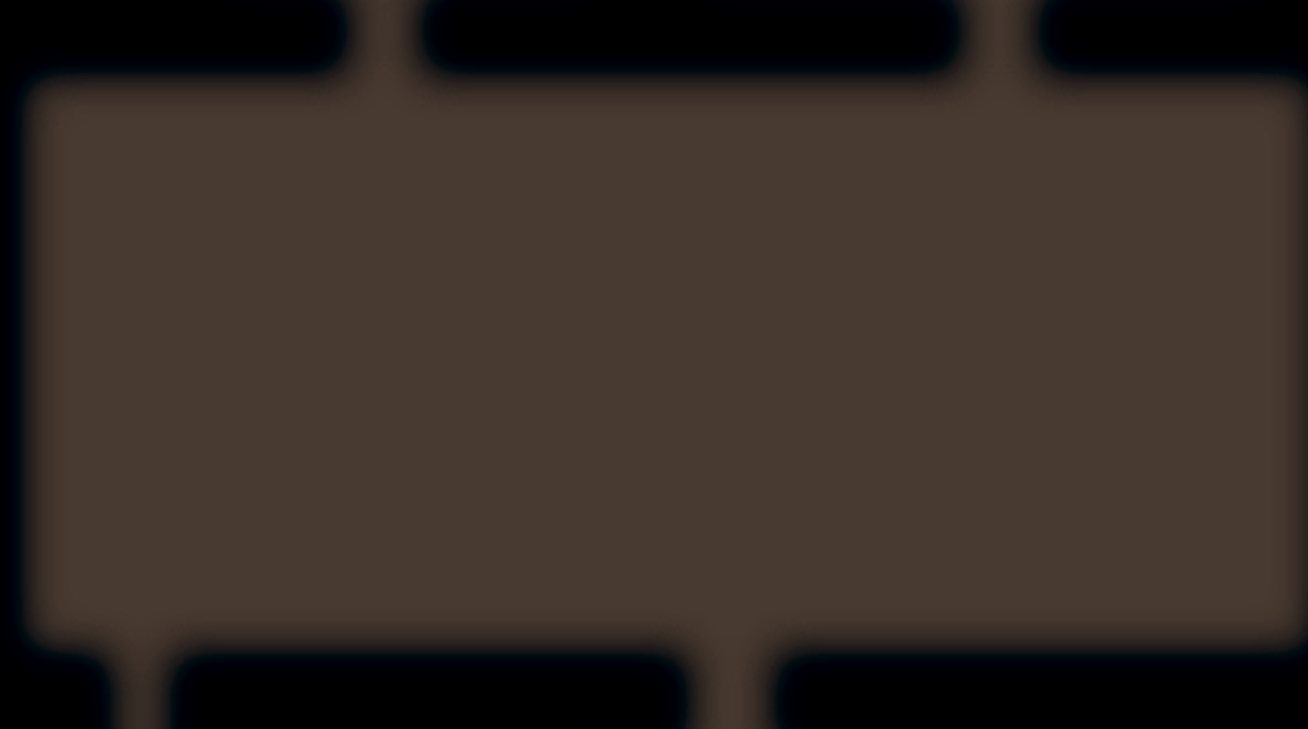
\includegraphics[width=0.45\textwidth, height=40mm]{images/nonPaused.png}
            & 
            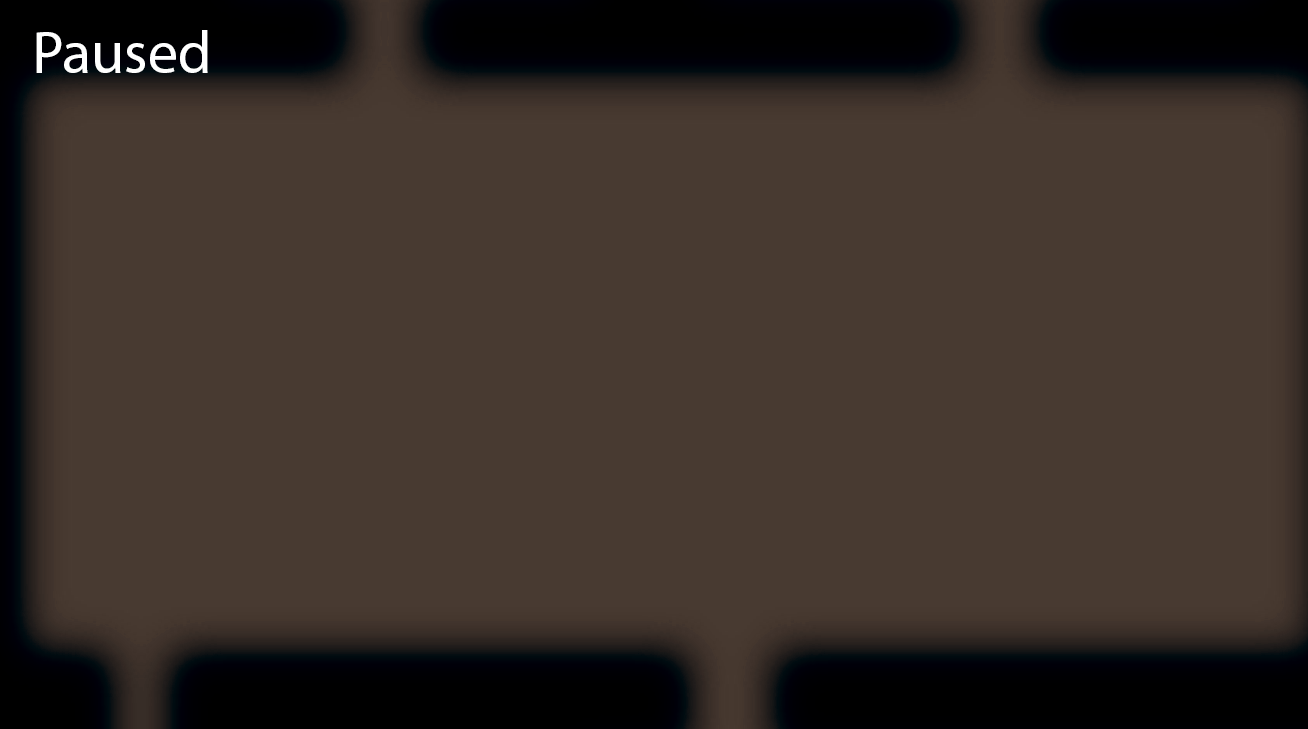
\includegraphics[width=0.45\textwidth, height=40mm]{images/Paused.png}    
            \\
            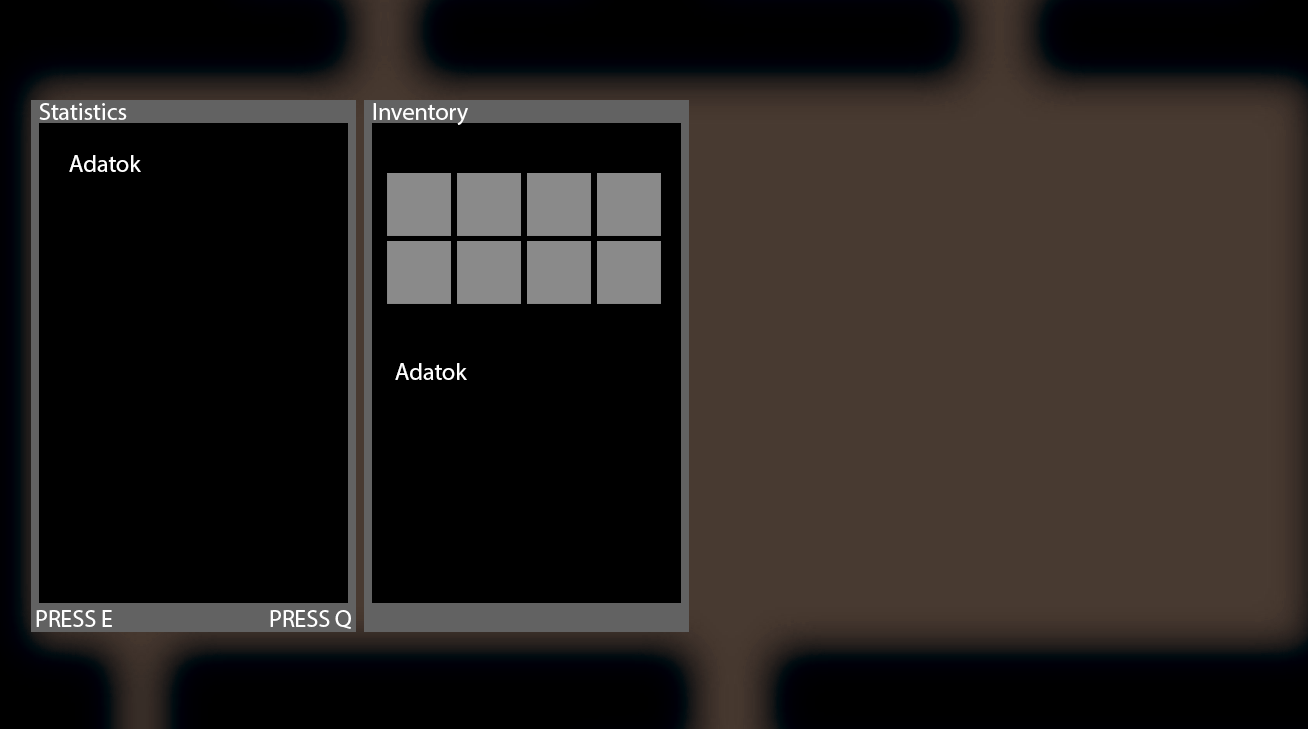
\includegraphics[width=0.45\textwidth, height=40mm]{images/Inventory.png}
            &
            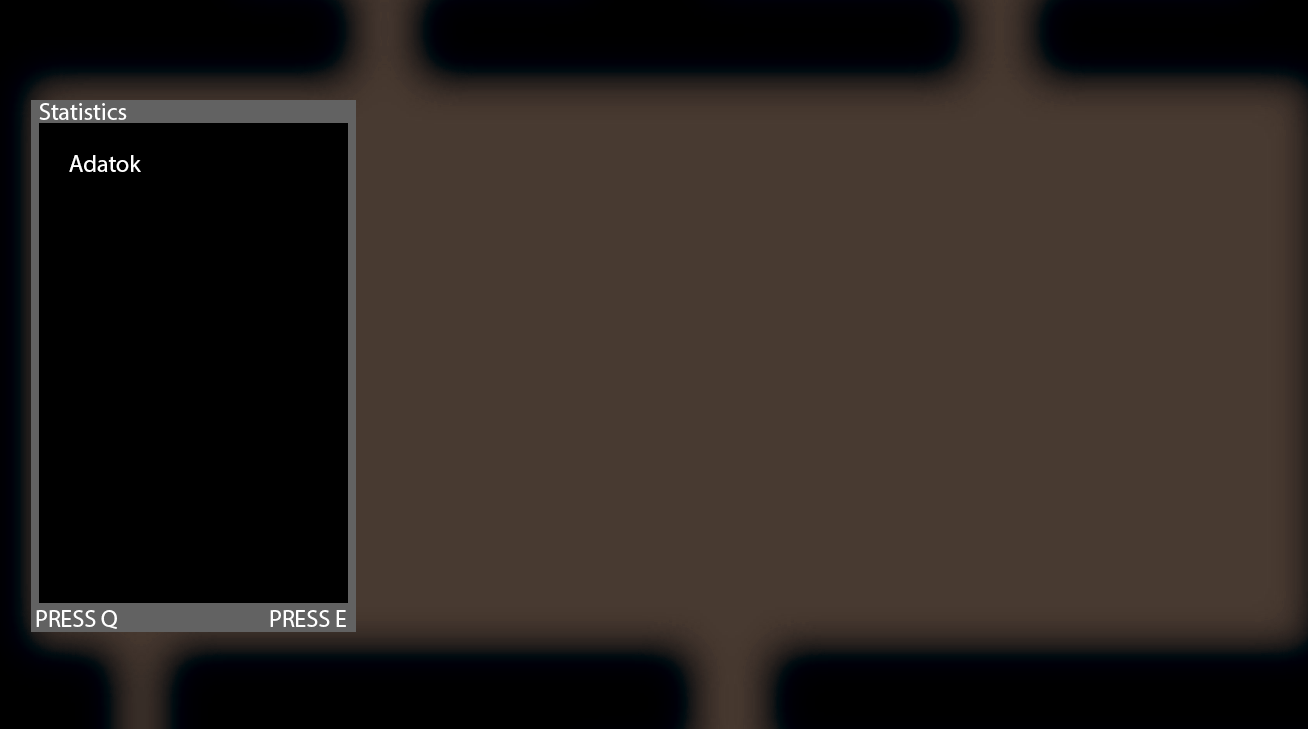
\includegraphics[width=0.45\textwidth, height=40mm]{images/Statistics.png}
            \\
            \multicolumn{2}{c}{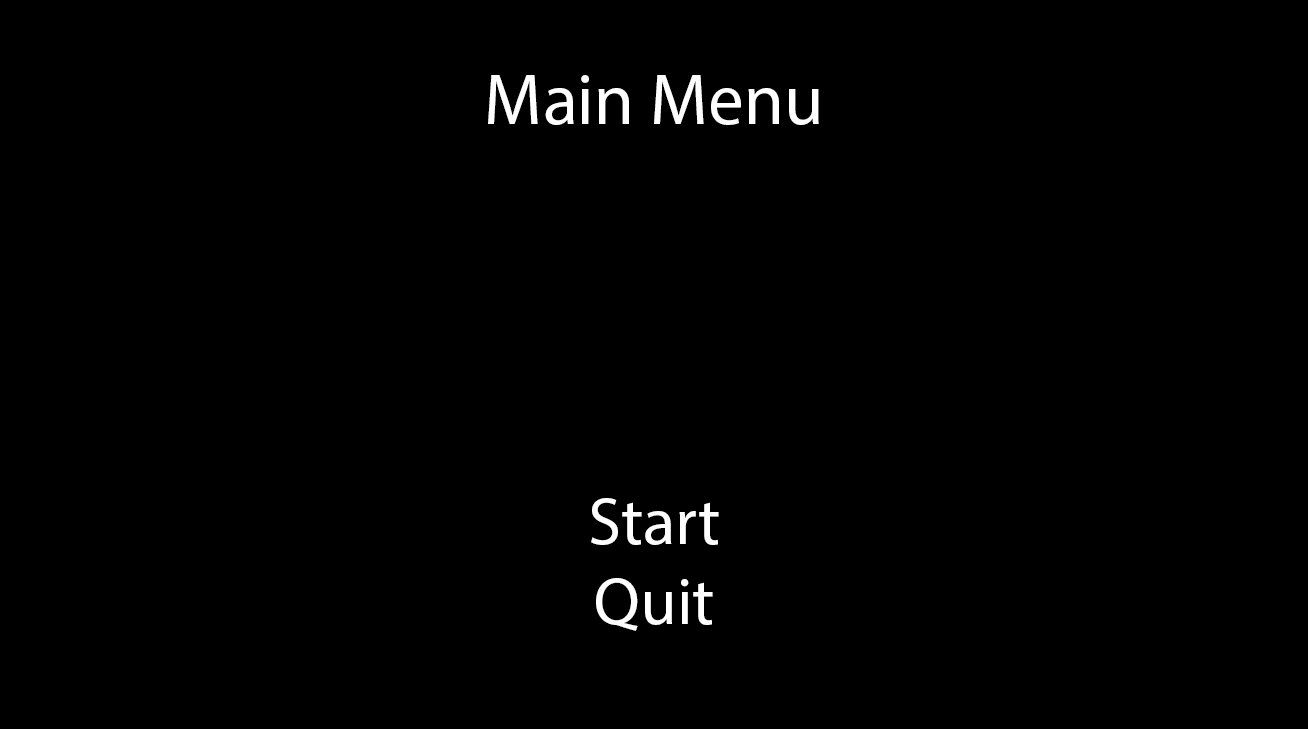
\includegraphics[width=0.45\textwidth, height=40mm]{images/MainMenu.png}}
        \end{tabular}
    \end{center}
    \caption{UI and Menu képernyőtervek}
    \label{tbl:tableofuiandmenu}
\end{figure}

\SubSection{Menü}

A szimulációs környezethez tartozik egy menü ablak. Ennek elemei az alábbiak.

\medskip

\noindent Szimuláció indítása előtt:
\begin{itemize}
    \item Középen felül a \textit{Main Menu} kiírását láhatjuk, alatta pedig 2 opcióból választhatunk (\ref{tbl:tableofuiandmenu}. ábra):
    \begin{itemize}
    \item[(1)] \textit{Start}, a kiválasztása esetén elindul a szimuláció,
    \item[(2)] \textit{Quit}, a szimulációs ablak bezárása.
    \end{itemize}
    \item A fenn említett két menüpont között a \texttt{W} (fel) és \texttt{S} (le) billentyűk lenyomásával navigálhatunk.
    \item Aláhúzva jelzi a felhasználónak, hogy mely menüpont van éppen kiválasztva.
    \item A különböző ablakok és UI elemek egy egyedi fontot használnak \cite{yosterislandfont}.
\end{itemize}

\noindent A szimuláció megállítása esetén:

\begin{itemize}
    \item A szimulációban a \texttt{P} billentyű lenyomásával képes a felhasználó megállítani a szimuláció menetét.
    \item A megállítást a bal felső sarokban kiírt fehér \textit{Paused} kiírás jelzi a felhasználó számára (\ref{tbl:tableofuiandmenu}. ábra).
    \item Ilyenkor az ágensek nem kapnak lehetőséget a lépésre, de a felhasználó képes a kamera mozgatására a nyilak segítségével.
    \item A felhasználó szintén képes az ágensek \textit{Statistics} ablakát megnyitni/bezárni a \texttt{C} billentyű megnyomásával, és előre/hátra lapozni az ágensek között a \texttt{Q} (balra) és \texttt{E} (jobbra) billentyűk megnyomásával, ha több van a szimulációban, mint 1.
    \item Ugyanígy képes megnyitni/bezárni az adott ágenshez tartozó \textit{Inventory} ablakot az \texttt{I} billentyű megnyomásával, ha látszódik az ágens statisztikája ablak.
    \item A \texttt{P} billentyű újonnan megnyomásával ott folytatódik a szimuláció, ahol abbamaradt (\ref{tbl:tableofuiandmenu}. ábra).
\end{itemize}

\Section{UI}
\label{UI}

A UI (\textit{User Interface}) foglalja magába az ágens szimulátor fő elemeit. A következőkben ennek az elemei, azok funkciói kerülnek felsorolásra.

\medskip

\noindent A szimuláció figyelésére szolgáló UI ablakok, amelyek a szimuláció kezdete után a képernyőn jelennek meg, a következők:

\begin{itemize}
    \item \textit{Statistics}: A \texttt{C} billentyű megnyomására megjelenik az első számú ágens Statistics ablaka (\ref{tbl:tableofuiandmenu}. ábra).
    \item \textit{Inventory}: Az \texttt{I} billentyű megnyomására megjelenik az az adott ágens \textit{Inventory} oldala (\ref{tbl:tableofuiandmenu}. ábra).
    \item \textit{Health Point}: Az ágens életerejét jeleníti meg.
\end{itemize}

\SubSection{Statistics}

\begin{itemize}
    \item Egy adott ágens adatának a kiolvasásának az eredményeit megjelenítő UI ablak. 
    \item A szimulációban megállítástól függetlenül a \texttt{C} billentyű megnyomására jelenik meg és tűnik el.
    \item Megnyitásakor mindig a még szimulációban létező ágensek közül az első számú ágens adait fogja visszaadni.
    \item A vizsgálandó ágens elpusztulásakor a még létező ágensek közül az új első számú ágens adatait fogja visszaadni.
    \item Ezen az ablakon a következő ágens adatokat írja ki:
    \begin{itemize}
    \item \textit{Sorszám}: Az ágens sorszámát adja vissza.
    \item \textit{HP} (életerő): Az ágens aktuális életerejét adja vissza.
    \item \textit{Erő} (str) Az ágens aktuális str értékét adja vissza.
    \item \textit{Kitartás} (vit): Az ágens aktuális vit értékét adja vissza.
    \item \textit{Kitérés} (eva): Az ágens aktuális eva értékét adja vissza.
    \item \textit{Pontosság} (acc): Az ágens aktuális acc értékét adja vissza.
    \end{itemize}
    Ezek a számok változhatnak az alapján, hogy milyen felszerelést hord az adott ágens.
    \item Új tárgy felvételénél, ha úgy ítéli, hogy jobb, mint az általa hordott azonos típusú tárgy, akkor lecseréli, és ennek megfelelően frissülnek a statisztikái.
\end{itemize}

\SubSection{Inventory}

\begin{itemize}
    \item Nem nyitható meg, ha nincs még megnyitva egy tetszőleges ágens \textit{Statistics} ablaka (\ref{tbl:tableofuiandmenu}. ábra).
    \item Megnyitásakor annak az ágensnek az \textit{Inventory}-ja lesz látható, amelyiknek a \textit{Statistics} oldala nyitva van.
    \item A \textit{Statistics} oldalon az előre/hátra lépés esetén az \textit{Inventory} az újonnan szemügyre vett ágens \textit{Inventory}-ját fogja megjeleníteni a felhasználó számára.
    \item Az \textit{Inventory}-ban a következő típusú tárgyak találhatóak meg:
    \begin{itemize}
    \item \textit{Armor} (páncél): Páncélként hordható tárgy, 4 alapstatisztikát tartalmaz.
    \item \textit{Helmet} (sisak): Sisakként hordható tárgy, 4 alapstatisztikát tartalmaz.
    \item \textit{Weapon} (fegyver): Fegyverként hordható tárgy, 4 alapstatisztikát tartalmaz.
    \item \textit{Key} (kulcs): Ajtó kinyitásához szükséges tárgy.
    \end{itemize}
    \item Az \textit{Inventory}-ban a \texttt{WASD} billentyűk lenyomásával választhatjuk ki, hogy mely \textit{Inventory} helyet akarjuk megnézni.
    \item A fehér üres négyzet jelöli azt a helyett az \textit{Inventory}-ban, amelyet éppen szemügyre vesz a felhasználó.
    \item Ha felszerelés típusú az adott tárgy, akkor a nevét és a 4 alapstatisztika értékét írja ki.
    \item Ha nem felszerelés típusú az adott tárgy, akkor pedig a nevét írja ki.
\end{itemize}

\SubSection{Health Point}

\begin{itemize}
    \item Minden ágens fölött az aktuális életcsíkja (\textit{HP, Health Point}) jelenik meg automatikusan.
\end{itemize}

\newpage

\Section{Szimulációs környezet specifikálása}

A következőkben a szimulációs környezet modelljének, elemeinek a specifikálására kerül sor.

\subsection{Map}

A szimulációban az ágensek egy diszkrét négyzetrács felbontáson tudnak mozogni. Ennek a mérete rögzített, $50 \times 50$, és minden elemhez egy saját definiálású \texttt{block} típus tartozik.

Egy \texttt{block}-nak van típusa, amely egy egész számként reprezentálható. Ez a következő értékeket veheti fel:
\begin{itemize}
\item 0 típus: Üres, a \textit{map}-on nem elérhető területeket jelöli.
\item 1 típus: Fal, a bejárható területeket körbezáró fal, amelyen nem lehet átmenni.
\item 2 típus: Füves terület, az ágensek által bejárható területek.
\end{itemize}

Kinézeteiket \aref{tbl:Blocks} ábrán láthatjuk. 

\begin{figure}[h!]
    \begin{center}
        \begin{tabular}{ ccc}
            
\includegraphics[width=0.3\textwidth, height=60mm]{images/block_brick.png}
            & 
            
\includegraphics[width=0.3\textwidth, height=60mm]{images/block_grass.png}    
            & 
            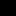
\includegraphics[width=0.3\textwidth, height=60mm]{images/block_empty.png}
            \\
        \end{tabular}
        \caption{Blokkok}
        \label{tbl:Blocks}
    \end{center}
\end{figure}

\medskip

Az $50 \times 50$-es mátrixon minden 2-es típusú blokkra helyezhetünk el egy objektumot. Az objektumok típusai az alábbiak lehetnek.

\begin{itemize}
\item \textit{Brick}: Egy mozgást korlátozó objektum. Nincs különösebb szerepe.
\item \textit{Chest}: \textit{End screen}-t előidéző tárgy, amely a szimuláció végét jelenti.
\item \textit{Door}: Egy mozgást korlátozó objektum. Kulccsal kinyitható az ágensek által.
\end{itemize}

Az objektumok egy részhalmaza olyan, hogy az ágensek fel tudják azokat venni az \textit{Inventory}-jukba, amelyek nem korlátozzák a mozgást. Ezek az alábbiak:
\begin{itemize}
\item \textit{Key},
\item \textit{Entity\_Armor\_01},
\item \textit{Entity\_Weapon\_01},
\item \textit{Entity\_Helmet\_01},
\item \textit{Entity\_Armor\_02},
\item \textit{Entity\_Weapon\_02},
\item \textit{Entity\_Helmet\_02}.
\end{itemize}

Kinézeteiket a \ref{tbl:Equipable items}. ábrán láthatjuk.

\begin{figure}[h!]
    \begin{center}
        \begin{tabular}{ | c | c | c | }
            \hline
            
\includegraphics[width=0.3\textwidth, height=60mm]{images/Entity_Armor_01.png}
            & 
            
\includegraphics[width=0.3\textwidth, height=60mm]{images/Entity_Helmet_01.png}    
            & 
            
\includegraphics[width=0.3\textwidth, height=60mm]{images/Entity_Weapon_01.png}
            \\
            \hline
            
\includegraphics[width=0.3\textwidth, height=60mm]{images/Entity_Armor_02.png}
            & 
            
\includegraphics[width=0.3\textwidth, height=60mm]{images/Entity_Helmet_02.png}    
            & 
            
\includegraphics[width=0.3\textwidth, height=60mm]{images/Entity_Weapon_02.png}
            \\
            \hline
        \end{tabular}
        \caption{Item sets}
        \label{tbl:Equipable items}
    \end{center}
\end{figure}

Szimuláció kezdetekor megtörténik a \textit{map} beolvasása. Ezt követően minden 2-es típusú blockra helyezhetünk el egy ágenst.
\begin{itemize}
    \item \textit{EntityFaction0}: 0-es számú csapatban lévő ágens.
    \item \textit{EntityFaction1}: 1-es számú csapatban lévő ágens.
\end{itemize}

A szimulációs környezetben adott számú elemet helyezünk le. Konkrétan az alábbi számú és típusú elemek kerülnek rá:
\begin{itemize}
    \item 18 szoba, 
    \item 25 ajtó,
    \item 25 kulcs,
    \item 4 ágens,
    \item 10 felvehető tárgy,
    \item 2 láda,
    \item 12 oszlop.
\end{itemize}

\SubSection{Szobák és folyosók}

A \textit{map}-en szobák és folyosók alakíthatók ki, de nem tetszőleges módon. Az alábbi szabályrendszer írja le, hogy milyen feltételek szerint helyezheti le ezeket a program.
\begin{itemize}
\item A szobákat több szomszédos cellák alkotják.
\item A szobákat folyosók kötik össze, amelyeket pontosan kettő cellával szomszédos cellák alkotnak.
\item Minden szomszédos szobát egy ajtó választ el egymástól.
\item A szobák celláin korlátozottan helyezkedhetnek el oszlopok, amely a cellát nem bejárható cellává alakítja át, és korlátozza a látást.
\item Minden szoba tartalmaz legalább 1 kulcsot, amely elősegíti a \textit{map} bejárhatóságát az ágensek által.
\end{itemize}

\SubSection{További map-re vonatkozó szabályok}

A \textit{map} szobák és folyosók összessége, ahol a szobák alakjánál törekszünk a négyzet alakú szobák elkerülésére. A folyosók általában rövidek és egy szobából akár több is nyílhat egy adott szobára.
A \textit{map} blokkokból épül fel. Blokkok típusát egy $[0, 2]$ intervallumon belüli számok jelölik.
Ezek az adatok a szimuláció kezdetekor kerülnek beolvasásra a \texttt{world01.txt}-ből.

A szobákban és a folyosókban bejárható terület egy mátrixhoz hasonló, amely celláit blokkoknak nevezzük.

Minden blokkhoz tartoznak további adatok, úgy mint:
\begin{itemize}
    \item $X$ koordináta (Integer),
    \item $Y$ koordináta (Integer).
\end{itemize}

\noindent Fontosabb kizáró feltételek:
\begin{itemize}
    \item Ajtó csak szoba és a folyosó, vagy szoba és a szoba között létezzen.
    \item Folyosóból ne nyíljon ajtó folyosóra.
    \item Két különböző folyosó ne érjen össze.
    \item Nem lehet olyan cellára mozgást kizáró objektumokat letenni, amely lehetetlenné teszi a \textit{map} egy tetszőleges pontjáról a \textit{map} egy másik tetszőleges pontjára való eljutását.
\end{itemize}

\Section{Tárgyak}

A tárgyakhoz a következő fontosabb adatok tartoznak:
\begin{itemize}
    \item \textit{name} (String): Az adott tárgyat bemutató név.
    \item \textit{typeName} (String): A tárgyak tartalmaznak tárgy típus nevet, például: Armor, Helmet, Key... stb.
    \item \textit{type} (Integer): A Key tárgy a 0 típusú, amíg minden hordható tárgy a 2 típus számot tartalmazza,
    \item \textit{str} (Integer): a tárgy ereje (\textit{strength}),
    \item \textit{vit} (Integer): a tárgy kitartása (\textit{vitality}),
    \item \textit{eva} (Integer): a tárgy kitérés (\textit{evasion}),
    \item \textit{acc} (Integer): a tárgy pontosság (\textit{accuracy}).
\end{itemize}
Az ágens által hordható tárgyaknak van valós \textit{str}, \textit{vit}, \textit{eva} és \textit{acc} értéke.

\Section{Tárgy nevek}

Ágens által használható felszerelési tárgy, amely statisztikát ad, amelyek hozzáadódnak, illetve kivonódnak az ágens jelenlegi statisztikáiból. Ezek értékeit \aref{tab:stats}. táblázatban láthatjuk. A tárgyak kinézetét a szimulációban pedig \ref{tbl:Equipable items}. ábrán láthatjuk, ahol a felső sor a 01 tárgyakat, a második sor a 02 tárgyakat foglalja össze.

\begin{table}[h!]
\centering
\caption{Tárgyak statisztikái}
\label{tab:stats}
\medskip
\begin{tabular}{|l|cc|cc|cc|cc|}
\textit{name} &
\multicolumn{2}{c|}{\textit{str}} &
\multicolumn{2}{c|}{\textit{vit}} &
\multicolumn{2}{c|}{\textit{eva}} &
\multicolumn{2}{c|}{\textit{acc}} \\
&
min & max &
min & max &
min & max &
min & max \\
\hline
Entity\_Helmet\_01 &
1 & 2 & 1 & 2 & 1 & 2 & 1 & 2 \\
Entity\_Helmet\_02 &
0 & 3 & 0 & 3 & 0 & 3 & 0 & 3 \\
Entity\_Armor\_01 &
1 & 2 & 1 & 2 & 1 & 2 & 1 & 2 \\
Entity\_Armor\_02 &
0 & 3 & 0 & 3 & 0 & 3 & 0 & 3 \\
Entity\_Weapon\_01 &
1 & 2 & 1 & 2 & 1 & 2 & 1 & 2 \\
Entity\_Weapon\_02 &
0 & 3 & 0 & 3 & 0 & 3 & 0 & 3 \\
\hline
\end{tabular}
\end{table}

\SubSection{Kulcs}

Celláról szerezhetőek meg.
Szerepük az ajtók kinyitása az ágens által.
Kulcsot tartalmazó ágens, elpusztulásakor a legutolsó helyén hagyja a kulcsot.

\Section{Ágensek}

A következő szakaszokban az ágensek tulajdonságai és a hozzájuk kapcsolódó számítási módok kerülnek részletezésre.

\SubSection{Statisztika}
\label{statisztika}

Az ágensek 4 alap statisztikával rendelkeznek.
Ez a 4 statisztika a következők: Erő, Kitérés, Kitartás, Pontosság. Az ágensek kezdő statisztikája fix 1.

Minden ágens a következő tárgyakkal kezd a szimulációban:
\begin{itemize}
    \item Entity\_Helm\_01,
    \item Entity\_Armor\_01,
    \item Entity\_Weapon\_01.
\end{itemize}

\subsection{Sebzés számlálás}

\label{számlálás}

A támadásnak két végkimenetele lehet:

\begin{itemize}
    \item \textit{Találat}: kiszámolódik a sebzés mértéke, és levonásra kerül a megfelelő ágens életerejéből.
    \item \textit{Eltévesztve}: nem történik meg a sebzés.
\end{itemize}

\SubSection{Statisztikák jelentősége}

Statisztikák jelentősége két különböző \textit{faction} változóval rendelkező ágens összetalálkozásánál látszódik meg.
Két fontosabb esetben játszik szerepet, az ágens statisztikája a fent említett találkozásnál.

Egy ágens egy másik ágensre mért csapásának sikeressége függ attól, hogy nagyobb-e a támadó ágens \textit{acc}, pontosság értéke, mint a támadást elszenvedő fél \textit{eva}, kitérés értéke.
Ha nagyobb a támadó ágens \textit{acc}, pontosság értéke, mint a támadott \textit{eva}, kitérés értéke, akkor 100\%-osan betalál a sebzése, azaz támadás betalálása következik be.
Ha nem nagyobb, akkor 20\% esélye van arra a támadott félnek, hogy ne kapjon semmilyen sebzést, azaz támadás eltévesztése következzen be.

Egy ágens egy másik ágensre mért csapásának a sebzése függ attól, hogy nagyobb-e a támadó ágens \textit{str}, erő értéke, mint a támadást elszenvedő fél \textit{vit}, kitartás értéke.
Ha nagyobb a támadó ágens \textit{str}, erő értéke, mint a támadott \textit{vit}, kitartás értéke, akkor 20\% esélye van arra a támadó félnek, hogy dupla sebzést mérjen be, ekkor a támadás nagysága nagy.
Ha nem nagyobb, akkor fixen 1 sebzést okoz a támadása, ekkor a támadás nagysága normál.

\SubSection{Elsődleges tulajdonságai}

Az ágens létrejöttekor kerül megadásra általunk.

\begin{itemize}
    \item str (Integer): az ágens ereje (\textit{strength}),
    \item vit (Integer): az ágens kitartás (\textit{vitality}),
    \item eva (Integer): az ágens kitérés (\textit{evasion}),
    \item acc (Integer): az ágens pontosság (\textit{accuracy}),
    \item maxLife (Integer): az ágens maximális életereje
    \item faction: (Integer): Lehet 0,1. Fontos változó a combat létrejöttéhez.
    \item healTurn: (Integer): Változó, amely azt tárolja, hogy melyik kör végén lesz HP regeneráció.
\end{itemize}

\SubSection{Kinézetet befolyásoló tényező}

\begin{itemize}
    \item Ágens állása. Látszódik, hogy milyen irányba néz.
    \item Az ágens \textit{faction} típusa.
\end{itemize}

\SubSection{Kommunikáció közöttük}

Ágensek bemenete, információ szerzése:
\begin{itemize}
    \item A hozzájuk szomszédos blokkokat vizsgálják, ha nem találnak semmit megvizsgálják az általuk érzékelhető blokkokat.
    \item A balra, jobbra, felfelé és lefelé irányban érzékelnek 2 blokknyi távolságra, ha nem gátolja meg valami az útjukat.
\end{itemize}

\noindent Ágensek belső memóriája a következőket tartalmazza:
\begin{itemize}
    \item \textit{Inventory} állapota.
    \item Karakter ablak állapota.
    \item Aktuális HP állapota.
    \item A blokkok \textit{hashMap} értékei (hogy hányszor volt az adott blokkokon, segít felderíteni a teljes térképet).
    \item Észlelt objektumok helyzete, típusa.
    \item \textit{Inventory}-ban tárolt tárgyak.
    \item Észlelt ágens értékei. (észlelt ágensek \textit{faction} értéke)
    \item Észlelt ágens helyzete ($X, Y$ koordináta).
\end{itemize}

\SubSection{Megfigyelési akcióik}

Információk feldolgozása:
\begin{itemize}
    \item Az \textit{Inventory} mérete és kihasználtsága. Ha elérte a maximum méretet nem képes az általa kívánt tárgyat felvenni.
    \item Karakter ablakban tárolt statisztikák számossága.
    \item Aktuális HP mennyiség. Adott Körönként fix HP visszatöltés történik meg (\ref{time}. szakasz).
    \item Az adott körben lehetséges lépesek \textit{hashMap} értékei vizsgálata, amelyek az adott blokk koordinátáit tárolják, és azt, hogy az adott ágens hányszor lépett rá az adott blokkra. (Szükséges azért, hogy idővel biztosan felfedezze az egész térképet.)
    \item Észlelt objektumok helyzete, típusa. Ezekből az információkból eldönti a prioritást, és ezáltal meghatározza, hogy mely irányba fog végül haladni.
    \item A nem használt tárgyak törlése, ha nem jobb a jelenleg hordottnál, ezáltal biztosítva, hogy ne teljen meg az \textit{Inventory} mérete.
    \item Ágens értékeiből leszűrt információk számításba vétele. (ellenség-e)
    \item Támadható ágensek közül a legkisebb életerővel rendelkező ágens támadását kezdeményezi.
\end{itemize}

\begin{figure}[h!]
    \begin{center}
        \begin{tabular}{ cc }
            
\includegraphics[width=0.70\textwidth, height=60mm]{images/endscreenblue.png}
            \\ 
            
\includegraphics[width=0.70\textwidth, height=60mm]{images/endscreenred.png}  
            \\
        \end{tabular}
        \caption{Záró képernyők (\textit{End screens})}
        \label{tbl:tableofendscreens}
    \end{center}
\end{figure}

\SubSection{Ágens tevékenységeinek a köre}

Az alábbiak bármely tevékenység végrehajtása, felhasználja az ágens körét.

\begin{itemize}

    \item Lépés. 
    
    \begin{itemize}
        \item A lépés akkor lehetséges, hogyha az ágens közvetlen közelében, azaz vagy az $X$ vagy az $Y$ koordinátájával szomszédos cellán nem tartózkodik mozgást korlátozó ágens/térbeli objektum, lásd itt: \nameref{object} szakasz.
    \end{itemize}

    \item Ajtó nyitás. 
    
    \begin{itemize}
        \item Szükséges az \textit{Inventory}-ban egy \textit{Key} nevű tárgy, amely a kulcs.
        \item Ha az ágens közvetlen közelében létezik ajtó, a nyitás akkor lehetséges.
        \item Nyitása után eltűnik az ajtó, és a kulcs az \textit{Inventory}-ból.
    \end{itemize}

    \item Láda nyitás. 
    
    \begin{itemize}
        \item Ha az ágens celláján létezik az ellenkező \textit{faction chest}-je, akkor a nyitás lehetséges.
        \item Ha nincs támadható ágens, akkor kinyitja.
        \item Megjelenő képernyő a kinyitása esetén vagy piros vagy kék (\ref{tbl:tableofendscreens}. ábra).
    \end{itemize}

    \item Felvétel. 
    
    \begin{itemize}
        \item Ha az \textit{Inventory}-ban van hely, akkor lehetséges.
        \item Ha az ágens celláján létezik valamilyen tárgy, ekkor a tárgyat a felvétel akcióval eltünteti a celláról, és az \textit{Inventory}-ba kerül.
    \end{itemize}

    \item Törlés. 
    
    \begin{itemize}
        \item Ha az \textit{Inventory}-ban van olyan tárgy, amely nem kulcs és nem hordott az ágens által, akkor lehetséges.
        \item Az ágens \textit{Inventory}-jából kitörli a tárgyat.
    \end{itemize}

    \item Felszerelés. 
    
    \begin{itemize}
        \item A felszerelés mindig lehetséges az ágens saját körében.
        \item Megvizsgálja, hogy az utoljára felvett tárgy statisztikái jobbak-e, mint az ő általa hordott azonos típusú hordható tárgy.
        \item Ha igen, felveszi azt, ezáltal megváltoztatva saját statisztikáit.
    \end{itemize}

    \item Támadás. 
    
    \begin{itemize}
        \item A támadás akkor lehetséges, hogyha az ágens közvetlen közelében, azaz vagy az $X$ vagy az $Y$ koordinátájával szomszédos cellán tartózkodik egy ellenséges ágens.
        \item Több ellenséges ágens esetén, a legkisebb életerővel rendelkező fogja támadni.
    \end{itemize}

\end{itemize}

\SubSection{Ágens fő céljai}

Az ágensnek alapvetően két célja van:
\begin{itemize}
    \item megtalálni az ellenséges \textit{chest}-et,
    \item elpusztítani az ellenséges ágenseket.
\end{itemize}

\SubSection{Ágens másodlagos céljai}

Az ágens szempontjából a következő tevékenységek végrehajtása szükségszerű, vagy előnyös lehet:
\begin{itemize}
    \item Tárgy felvétel,
    \item Tárgy hordása adott esetekben,
    \item Ajtó kinyitás,
    \item \textit{Inventory} menedzsment,
    \item Mindig a kevesebbszer bejárt blokkokat választani mozgáskor.
\end{itemize}

\begin{figure}[h!]
    \centering
    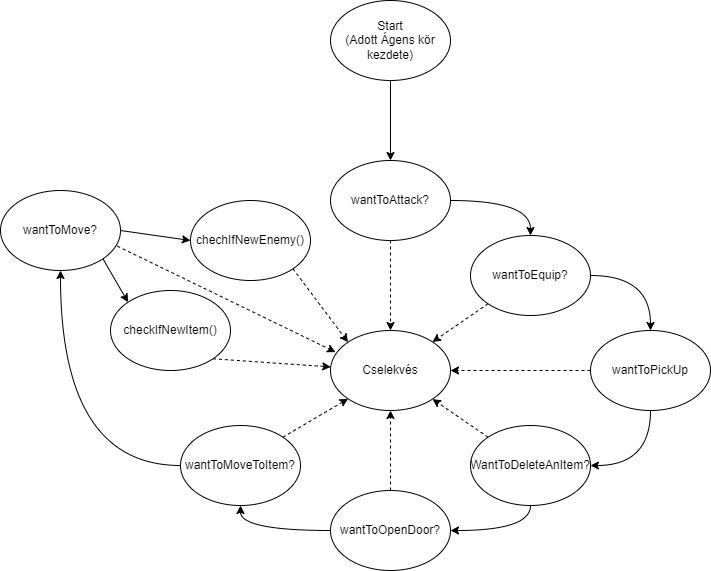
\includegraphics[scale=0.6]{images/agentfunction.png}
    \caption{\textit{Agent Action Priority} állapotgép modell}
    \label{fig:Priority}
\end{figure}

\SubSection{Ágens függvény}

\Aref{fig:Priority}. ábrán látható az ágens cselekvésének meghatározására szolgáló állapotgép gráfja, amely a szimuláció kezdetétől működik.
A csomópontok fontossági sorrendben a következők.
\begin{itemize}
    \item wantToAttack?
    
    \begin{itemize}
        \item Ha közvetlen közelében van egy ellenséges ágens, mindig azt az akciót választja, ahol támadást mér be az ellenséges ágensnek.
    \end{itemize}

    \item wantToEquip?
    
    \begin{itemize}
        \item Ha a legutoljára általa felvett tárgy statisztikái több statisztikát adnak összességében, mint az általa hordott azonos típusú tárgy, akkor lecseréli.
    \end{itemize}

    \item wantToPickUp?
    
    \begin{itemize}
        \item Ha az ágenset tartalmazó blokk-on létezik valamilyen felvehető tárgy az ágens által, akkor felveszi.
    \end{itemize}

    \item wantToDeleteAnItem?
    
    \begin{itemize}
        \item Ha az ágens \textit{Inventory}-ja tartalmaz olyan hordható tárgyat, amely nem jobb mint az általa hordott tárgy, akkor eltávolítja az\textit{Inventory}-jából.
    \end{itemize}

    \item wantToOpenDoor?
    
    \begin{itemize}
        \item Ha van kulcs nála, és a közvetlen közelében van egy ajtó, akkor az ajtó kinyitását választja.
    \end{itemize}

    \item wantToMoveToItem?
    
    \begin{itemize}
        \item Ha van olyan közvetlen közeli blokk az ágens szomszédjában, amelyre lehetséges a lépés, és tartalmaz valamilyen felvehető tárgyat,
        akkor összeveti az ágens és a felvenni kívánt tárgy koordinátáit, és az alapján eldönti milyen irányba mozogjon az ágens. 
    \end{itemize}

    \item newEnemy?

    \begin{itemize}
        \item Ez az eset akkor lép fel, ha semmilyen más cselekvést nem akart elvégezni az adott körben az ágens és lát a \textit{detectableBlocks}-on belül olyan blokkot,
        amely egy ellenséges ágenst tartalmaz. Ilyenkor a hozzá közeli blokkot választja ki következő lépésének.
    \end{itemize}

\newpage

    \item newItem?

    \begin{itemize}
        \item Ez az eset akkor lép fel, ha semmilyen más cselekvést nem akart elvégezni az adott körben az ágens, és lát a \textit{detectableBlocks}-on belül olyan blokkot,
        amely egy kívánt tárgyat tartalmaz, ilyenkor a hozzá közeli blokkot választja ki következő lépésének.
    \end{itemize}

    \item wantToMove?
    
    Ez az eset akkor lép fel, ha semmilyen más cselekvést nem akart elvégezni az adott körben az ágens.

    \begin{itemize}
        \item A lehetséges blokkok közül kiválasztja azt a blokkot a következő lépésének, amelyen még nem volt soha.
        \item Ha több olyan lehetséges blokk van, amelyre léphet, akkor véletlenszerűen választ egyet a lehetőségek közül.
        \item Ha nincs egy olyan blokk se, ahol ne lett volna már, akkor a legkevesebbszer bejárt blokkot fogja választani.
        \item Ha több legkevesebbszer bejárt blokk létezik a lehetséges blokkok közül, akkor véletlenszerűen választ egyet a lehetőségek közül.
    \end{itemize}
\end{itemize}

\Section{Cél Tárgy}

Egy térkép teljesítéséhez szükséges tárgy, amely egy \textit{chest}, láda. A kék \textit{faction}-nek a piros ládát, a piros \textit{faction}-nek a kék ládát kell elérnie és interakcióba lépni vele. (Ezek megjelenítését \aref{tbl:Chests}. ábrán láthatjuk.)
A térképen a ládák az ellenkező \textit{faction} típusú ágensek kezdő szobájában helyezkedik el.

\begin{figure}[h!]
    \begin{center}
        \begin{tabular}{ | c | c | }
            \hline
            
\includegraphics[width=0.3\textwidth, height=60mm]{images/chest_0.png}
            & 
            
\includegraphics[width=0.3\textwidth, height=60mm]{images/chest_1.png}    
            \\
            \hline
        \end{tabular}
        \caption{Ládák (\textit{Chests})}
        \label{tbl:Chests}
    \end{center}
\end{figure}

\Section{Támadás}

A szimulációban 1-es \textit{faction} változójú ágens és 2-es \textit{faction} változójú ágens közötti életerő elvétel a szomszédos cellából lehetséges. A támadás lehet betalált vagy elvétett. A támadás nagysága lehet normális vagy nagy.

\Section{Felhasználói felület}

A felhasználói felületen az elvégezhető műveletek különféle előfeltételekhez (prekondíciókhoz) vannak kötve. A műveleteknek van általános működése, illetve bekövetkezhet valamilyen alternatív és kivételes eset is.

A következő alpontokban a felhasználó által végrehajtható műveletek áttekintésére kerül sor, benne felsorolva azok prekondícióit, posztkondícióit, továbbá az eseteket.

\subsection{Pause}

\begin{itemize}
    \item prekondíció: A szimulációs ablakban vagyunk.
    \item általános működés: Megnyomjuk a \texttt{P} gombot.
    \item alternatív esetek: Rossz tevékenység következik be.
    \item posztkondíció: Megjelent a \textit{Paused} kiírás bal fent.
    \item kivételes esetek: Nem állt meg a játékmenet.
\end{itemize}

\subsection{Inventory}

\begin{itemize}
    \item prekondíció: A szimulációs ablakban vagyunk, és meg van már nyitva egy tetszőleges \textit{Statistics} ablak.
    \item általános működés: Megnyomjuk az \texttt{I} gombot.
    \item alternatív esetek: Rossz ablak nyílik meg.
    \item posztkondíció: Megnyílt az \textit{Inventory} ablak.
    \item kivételes esetek: Nem nyílt meg az ablak.
\end{itemize}

\subsection{Statistics}

\begin{itemize}
    \item prekondíció: A szimulációs ablakban vagyunk.
    \item általános működés: Megnyomjuk a \texttt{C} gombot.
    \item alternatív esetek: Rossz ablak nyílik meg.
    \item posztkondíció: Megnyílt a létező ágensek közül a legelső \textit{Statistics} ablak.
    \item kivételes esetek: Nem nyílt meg az ablak.
\end{itemize}

\Section{Akadályok}
\label{object}

A következőkben a térképen található mozgást kizáró objektumok kerülnek bemutatásra.

\SubSection{Brick}
\label{brick}

A \textit{Brick} egy oszlop, amely a térkép beolvasása után kerül bizonyos cellákra. A kinézetéhez felhasznált kép \aref{tbl:Brick}. ábrán látható.

Az oszlopoknak semmilyen különleges funkciója nincs azonkívül, hogy a térkép komplexitását kívánja növelni azzal,
hogy mozgást és látást korlátozó szerepet lát el.

\begin{figure}[h!]
    \begin{center}
        \begin{tabular}{c}
            
\includegraphics[scale=10]{images/object_brick.png}
        \end{tabular}
        \caption{Brick}
        \label{tbl:Brick}
    \end{center}
\end{figure}

\subsection{Zárt ajtó}

Az ajtók a térkép beolvasása után kerülnek bizonyos cellákra.
Az ajtók mozgást korlátozó szerepet töltenek be, ha nincs az ágensnél kulcs. Ha van, akkor a szomszédos blokkból kinyithatja az ajtókat.
Ahogyan az \textit{brick}-ek, a zárt ajtók is a térkép komplexitását kívánja növelni. A kulcsról és az ajtóról láthatunk egy képet \aref{tbl:Key and Door}. ábrán.

\begin{figure}[h!]
    \begin{center}
        \begin{tabular}{ | c | c | }
            \hline
            
\includegraphics[scale=10]{images/key.png}
            & 
            \includegraphics[scale=10]{images/Door.png}    
            \\
            \hline
        \end{tabular}
        \caption{Key and Door}
        \label{tbl:Key and Door}
    \end{center}
\end{figure}


\Section{Idő}
\label{time}

A szimuláció egy diszkrét idejű rendszert modellez. Minden ágens által végrehajtott művelet során egy-egy időegység telik el.

Minden 5. kör után, 1 HP-t töltenek vissza az ágensek, ha kisebb az aktuális életerejük, mint a maximális.
Ha egy ágens elvégez egy akciót, akkor az irányítás átkerül egy másik ágensre.

\Section{Kamera}

A szimulációban modellezett virtuális teret valahogyan láthatóvá kell tenni. Ezt egy felülnézetes kamera formájában képzelhetjük el. A kamera mozgására néhány egyszerű szabály vonatkozik.
\begin{itemize}
    \item A kamera blokkról blokkra képes haladni 3 koordináta meglépésével.
    \item A kamera képes mozogni, akkor is ha a játékmenet szünetel (\textit{Paused}).
\end{itemize}

\Section{Irányítás}

A korábbiakban már érintőlegesen szó esett a szimulációs környezetben használt billentyűkről, az azokkal kiváltott eseményekről. A következő felsorolásban áttekintésképpen láthatjuk ezeket egy helyen.
\begin{itemize}
    \item Kamera mozgatása: \texttt{WASD},
    \item Ágens \textit{Statistics} ablak megnyitása/bezárása: \texttt{C},
    \item Ágensek \textit{Statistics} ablaka közötti lépegetés: \texttt{Q} (hátra), \texttt{E} (előre),
    \item Adott ágens \textit{Statistics} oldalához tartozó \textit{Inventory} megnyitása/bezárása: \texttt{I}.
\end{itemize}








